\documentclass[aspectratio=169,12pt]{beamer}
\usepackage{pgfpages}
\mode<presentation> {
  \usetheme{metropolis}
}

\usepackage{lipsum}
% \usepackage[colorgrid,gridunit=pt,texcoord]{eso-pic}
\usepackage[absolute,overlay]{textpos}
\usepackage{pythonhighlight}
\usepackage[absolute,overlay]{textpos}
\usepackage{url}
\usepackage{caption}
\usepackage{hyperref}
\usepackage[
    type={CC},
    modifier={by},
    version={3.0},
]{doclicense}
\usepackage[whole]{bxcjkjatype}
\usepackage{todonotes}
\usepackage{multimedia}

\setbeamertemplate{note page}{\pagecolor{yellow!5}\vfill\insertnote\vfill}
\setbeameroption{show notes on second screen=right}

\lstset{
language = Python,
breaklines = true,
basicstyle=\fontsize{7}{7}\selectfont\ttfamily,
commentstyle = {\itshape \color[cmyk]{1,0.4,1,0}},
keywordstyle = {\bfseries \color[cmyk]{0,1,0,0}},
stringstyle = {\ttfamily \color[rgb]{1,0,0}},
frame = single,
}
\hypersetup{
colorlinks=true,
}

\title{Visualize 3D scientific data in a Pythonic way like matplotlib}

\begin{document}
\author{Tetsuo Koyama}
\institute{PyVista developer team}

\frame{\titlepage}
\note{
Hi my name is Tetsuo Koyama. Today I will talk about the title "Visualize 3D scientific data in a Pythonic way like matplotlib".

こんにちは、Tetsuo Koyamaです。本日は、「Pythonicに3次元データを可視化しよう」というタイトルでお話します。
}

\begin{frame}[fragile]
\begin{textblock*}{350pt}(50pt, 20pt)
\begin{block}{Who am I?}
\note{
Let me introduce myself first.

まずは自己紹介をさせてください。

}
\end{block}
\end{textblock*}
\begin{textblock*}{350pt}(50pt, 70pt)

\includegraphics[width=0.25\linewidth]{tkoyama010.png}
\end{textblock*}
\begin{textblock*}{350pt}(50pt, 170pt)

\includegraphics[width=0.05\linewidth]{twitter-5662063_1280.png}
\end{textblock*}
\begin{textblock*}{350pt}(70pt, 175pt)
\href{https://twitter.com/tkoyama010}{@tkoyama010}
\end{textblock*}
\begin{textblock*}{350pt}(50pt, 200pt)
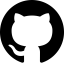
\includegraphics[width=0.05\linewidth]{github.png}
\end{textblock*}
\begin{textblock*}{350pt}(70pt, 205pt)
\href{https://github.com/tkoyama010}{@tkoyama010}
\end{textblock*}
\begin{textblock*}{350pt}(150pt, 25pt)
\begin{itemize}
\item Scientific simulation software engineer.
\note{
I am mechanical simulation software engineer in my careers.

私は科学シミュレーションのソフトウェアエンジニアとして働いています。

}
\item Stuff of Scipy Japan 2020.
\note{
And I was a staff of Scipy Japan 2020.

そして、Scipy Japan 2020のスタッフを務めました。

}
\item PyVista developer team member.
\note{
Also I am a member of PyVista developer team.

また、PyVista開発チームのメンバーでもあります。

}
\item Science, Python, Anime, and Manga.
\note{
I love Science, Python, Anime and Manga.

科学、Python、アニメ、マンガが大好きです。

}
\end{itemize}
\end{textblock*}
\begin{textblock*}{350pt}(200pt, 120pt)
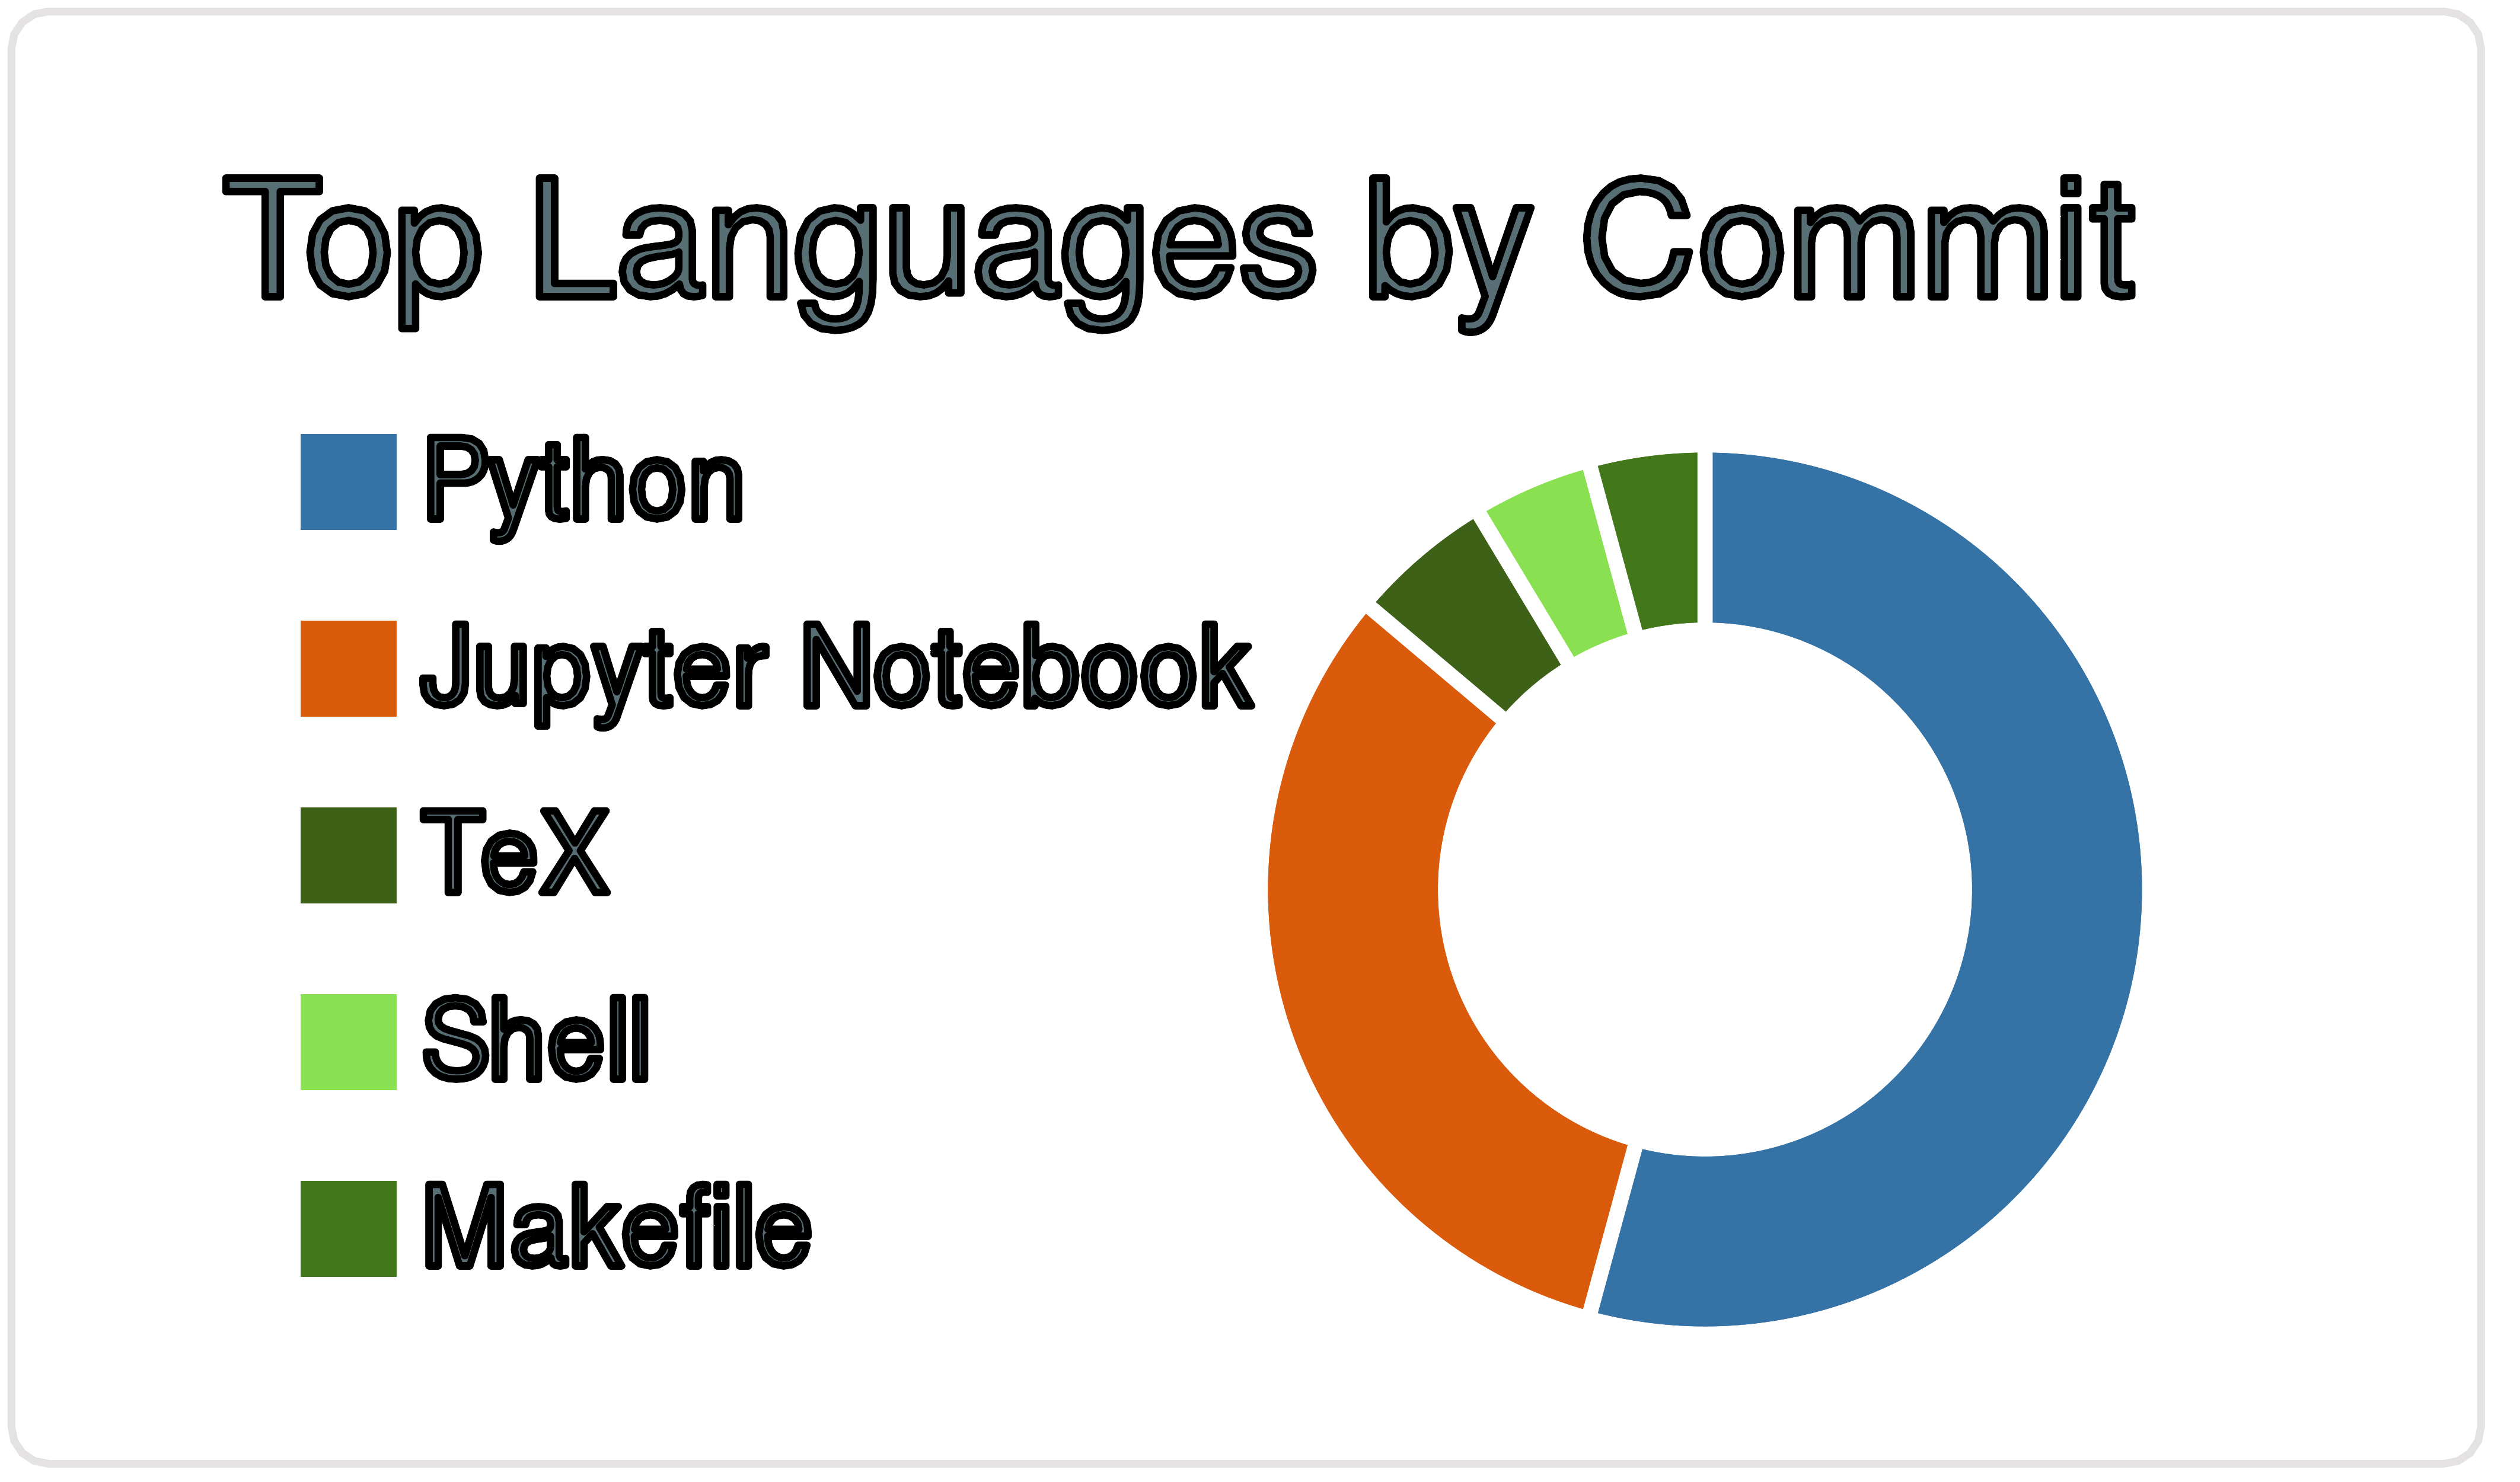
\includegraphics[width=0.50\linewidth]{2-most-commit-language.png}
\end{textblock*}
\note{
My Twitter and Github accounts are \href{https://twitter.com/tkoyama010}{@tkoyama010}.

私のTwitterとGithubのアカウントは\href{https://twitter.com/tkoyama010}{@tkoyama010}です。

}
\note{
Please follow me if you like this presentation.

このプレゼンテーションを気に入っていただけたら、ぜひフォローしてください。
}
\end{frame}

\begin{frame}[fragile]
\begin{textblock*}{800pt}(50pt, 10pt)
\begin{block}{What we want to do is using VTK like matplotlib in PyVista.}
\note{
Do you want to visualize 3D data in a Pythonic way like matplotlib?
If you want, this slides is for you.
This slides is the introduction of \href{https://pypi.org/project/pyvista/}{PyVista}. It is

}
\begin{itemize}
\item "VTK for humans"\: a high-level API to the Visualization Toolkit (VTK)
\note[item]{
"VTK for humans"\: a high-level API to the Visualization Toolkit (VTK).
}
\item 3D plotting made simple and built for large/complex data geometries
\note[item]{
3D plotting made simple and built for large/complex data geometries
}
\item mesh data structures and filtering methods for spatial datasets
\note[item]{
mesh data structures and filtering methods for spatial datasets

% matplotlibのようにPythonicな方法で3Dデータを視覚化したいと思ったことはありませんか?
% このスライドはそんなあなたのためのものです。
% このスライドでは、\href{https://pypi.org/project/pyvista/}{PyVista}と呼ばれるライブラリを紹介します。
% このライブラリには3つの特徴があります。
% 1つ目は"人間のためのVTK"\: 可視化ツールキット(VTK)の高レベルAPIです。
% 2つ目は大規模/複雑なデータ形状に対応した、シンプルな3Dプロッティング機能です。
% 3つ目はメッシュデータと空間データのフィルタリングメソッドです。
}
\end{itemize}
\note{
VTK is an excellent visualization toolkit, and with Python bindings it should be able to combine the speed of C++ with the rapid prototyping of Python.
However, despite this VTK code programmed in Python generally looks the same as its C++ counterpart.
This module seeks to simplify mesh creation and plotting without losing functionality.
}
\end{block}
\end{textblock*}
\begin{textblock*}{800pt}(50pt, 150pt)
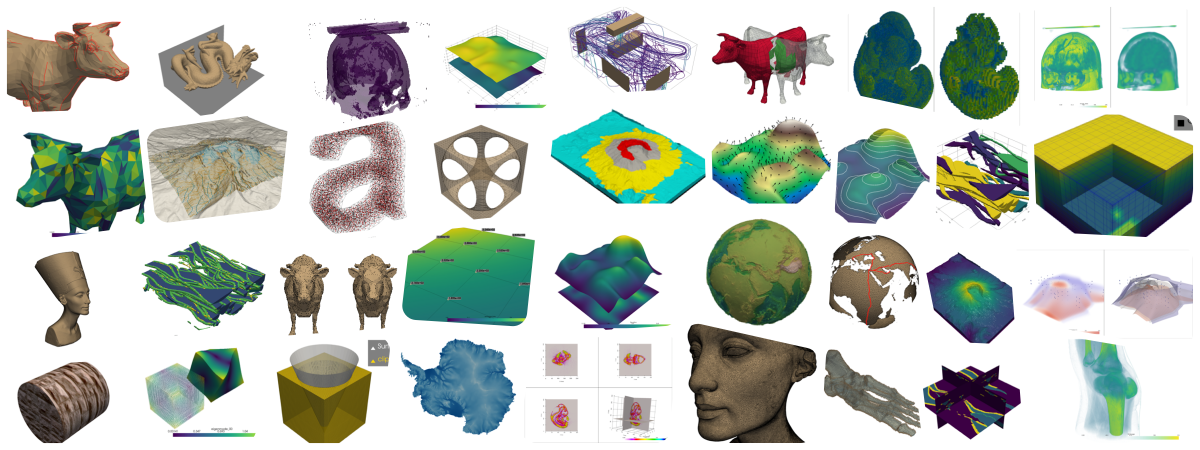
\includegraphics[width=0.50\linewidth]{pyvista_banner_small.png}
\end{textblock*}
\end{frame}

\begin{frame}[fragile]
\begin{textblock*}{800pt}(50pt, 10pt)
\begin{block}{In this slides you can learn.. }
\begin{itemize}
\item Pythonic interface to VTK’s Python bindings
\item Filtering/plotting tools built for interactivity
\item Direct access to common VTK filters
\item Intuitive plotting routines with matplotlib similar syntax
\end{itemize}
\end{block}
\end{textblock*}
\begin{textblock*}{800pt}(50pt, 110pt)
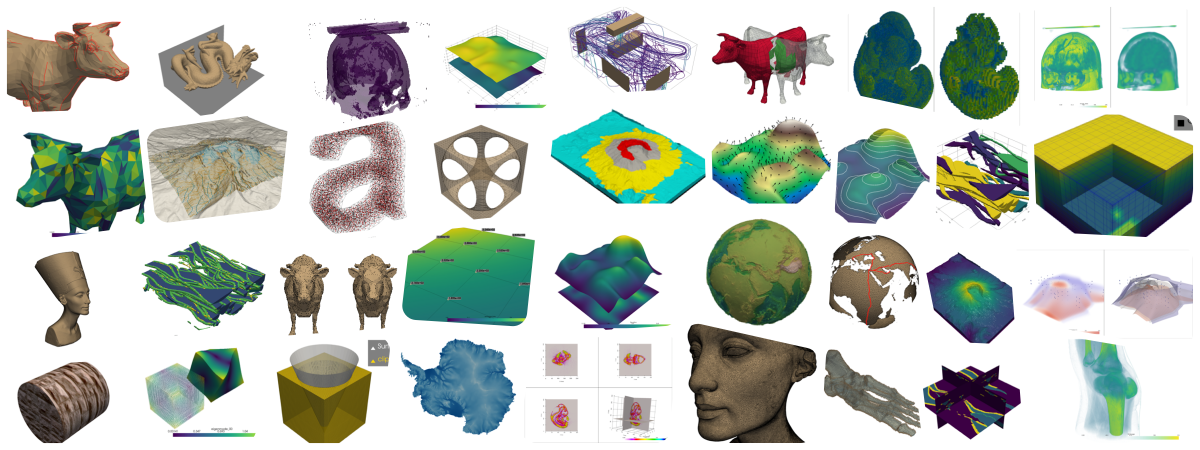
\includegraphics[width=0.50\linewidth]{pyvista_banner_small.png}
\end{textblock*}
\end{frame}
\note{
In this presentation, you can learn more about how PyVista wraps different VTK mesh types and how you can leverage powerful 3D plotting and mesh analysis tools. Highlights of the API include:

Pythonic interface to VTK’s Python bindings

Filtering/plotting tools built for interactivity (see Widgets)

Direct access to common VTK filters (see Filters)

Intuitive plotting routines with matplotlib similar syntax (see Plotting)

}
\begin{frame}[fragile]
\begin{textblock*}{350pt}(50pt, 10pt)
\begin{block}{Hello World!}
\lstinputlisting[caption=Hello World!, label=hello_world_code, firstline=1, lastline=100]{hello_world.py}
\end{block}
\end{textblock*}
\end{frame}
\note{
PyVista is a helper module for the Visualization Toolkit (VTK) that takes a different approach on interfacing with VTK through NumPy and direct array access.
This package provides a Pythonic, well-documented interface exposing VTK’s powerful visualization backend to facilitate rapid prototyping, analysis, and visual integration of spatially referenced datasets.
This module can be used for scientific plotting for presentations and research papers as well as a supporting module for other mesh dependent Python modules.
In Code Listing \ref{hello_world_code}, we demonstrate the "Hello World!" of \href{https://pypi.org/project/pyvista/}{PyVista}.
Basic step of \href{https://pypi.org/project/pyvista/}{PyVista} script is the following.
First, import \href{https://pypi.org/project/pyvista/}{PyVista}.
Then generate \href{https://dev.pyvista.org/getting-started/what-is-a-mesh.html}{mesh} and add it to
Plotter object using add mesh method.
This example also shows how to create a multi-window plotter by specifying the shape parameter.
The window generated is a two by two window by setting shape=(1, 3). Use the pyvista.BasePlotter.subplot() function to select the subplot you wish to be the active subplot.
And "add\_text" method add text to plot object in the top left corner by default.

コードリスト\ref{hello_world_code}では、\href{https://pypi.org/project/pyvista/}{PyVista}の "Hello World!" を行っています。
\href{https://pypi.org/project/pyvista/}{PyVista} スクリプトの基本ステップについて説明します。
まず、 \href{https://pypi.org/project/pyvista/}{PyVista} をインポートします。
次に \href{https://dev.pyvista.org/getting-started/what-is-a-mesh.html}{mesh} を生成して、それを
add meshメソッドを使用してPlotterオブジェクトに追加します。

}

\begin{frame}[fragile]
\begin{textblock*}{350pt}(50pt, 10pt)
\begin{block}{Hello World!}
\lstinputlisting[caption=Hello World!, label=hello_world_code, firstline=1, lastline=100]{hello_world.py}
\end{block}
\end{textblock*}
\end{frame}
\note{
PyVista is a helper module for the Visualization Toolkit (VTK) that takes a different approach on interfacing with VTK through NumPy and direct array access.
This package provides a Pythonic, well-documented interface exposing VTK’s powerful visualization backend to facilitate rapid prototyping, analysis, and visual integration of spatially referenced datasets.
This module can be used for scientific plotting for presentations and research papers as well as a supporting module for other mesh dependent Python modules.
In Code Listing \ref{hello_world_code}, we demonstrate the "Hello World!" of \href{https://pypi.org/project/pyvista/}{PyVista}.
Basic step of \href{https://pypi.org/project/pyvista/}{PyVista} script is the following.
First, import \href{https://pypi.org/project/pyvista/}{PyVista}.
Then generate \href{https://dev.pyvista.org/getting-started/what-is-a-mesh.html}{mesh} and add it to
Plotter object using add mesh method.
This example also shows how to create a multi-window plotter by specifying the shape parameter.
The window generated is a two by two window by setting shape=(1, 3). Use the pyvista.BasePlotter.subplot() function to select the subplot you wish to be the active subplot.
And "add\_text" method add text to plot object in the top left corner by default.

コードリスト\ref{hello_world_code}では、\href{https://pypi.org/project/pyvista/}{PyVista}の "Hello World!" を行っています。
\href{https://pypi.org/project/pyvista/}{PyVista} スクリプトの基本ステップについて説明します。
まず、 \href{https://pypi.org/project/pyvista/}{PyVista} をインポートします。
次に \href{https://dev.pyvista.org/getting-started/what-is-a-mesh.html}{mesh} を生成して、それを
add meshメソッドを使用してPlotterオブジェクトに追加します。

}
\begin{frame}[fragile]
\begin{textblock*}{350pt}(50pt, 10pt)
\begin{block}{Hello World!}
\end{block}
\end{textblock*}
\begin{textblock*}{350pt}(50pt, 50pt)
\begin{block}{}
\begin{figure}
\includegraphics[width=1.0\linewidth]{hello_world.png}
\caption{Hello World!\label{HelloWorldFigure}}
\end{figure}
\note{
And finally, we can check the render view (Figure \ref{HelloWorldFigure}) of PyVista using show method.

最後に、showメソッドを使って、PyVistaのレンダリングビュー(図 \ref{HelloWorldFigure})を確認します。
}
\end{block}
\end{textblock*}
\end{frame}

\begin{frame}[fragile]
\begin{textblock*}{350pt}(50pt, 10pt)
\begin{block}{Create tube from line}
\lstinputlisting[caption=Create tube, label=CreateTube, firstline=15, lastline=15]{tube.py}
\begin{figure}
\includegraphics[width=1.0\linewidth]{tube.png}
\caption{Line and tube\label{LineTubeFigure}}
\end{figure}
\end{block}
\end{textblock*}
\end{frame}
\note{
We can also make customize mesh like tube from line points using Tube function.

Tube関数を使用して、線の点から管のようなメッシュをカスタマイズすることもできます。
}

\begin{frame}[fragile]
\begin{textblock*}{200pt}(50pt, 10pt)
\begin{block}{Create PolyData}
\lstinputlisting[caption=Create PolyData, label=CreatePolyDataCode, firstline=12, lastline=29]{create-poly.py}
\end{block}
\end{textblock*}
\begin{textblock*}{350pt}(180pt, 50pt)
\begin{figure}
\includegraphics[width=0.5\linewidth]{create-poly.png}
\caption{Create PolyData \label{CreatePolyData}}
\end{figure}
\end{textblock*}
\end{frame}
\note{
You can also create PolyData (Triangulated Surface) objects from the NumPy arrays of vertices and faces if you want to further customize the mesh.

メッシュをさらにカスタマイズする場合は、頂点と面のNumPy配列からPolyData (Triangulated Surface) オブジェクトを作成することもできます。

A PolyData object can be created quickly from numpy arrays.

PolyDataオブジェクトは、numpy配列からすばやく作成できます。

The vertex array contains the locations of the points in the mesh and the face array contains the number of points of each face and the indices of the vertices which comprise that face.

頂点配列にはメッシュ内のポイントの位置が含まれ、面配列には各面のポイント数と、その面を構成する頂点のインデックスが含まれます。

}

\begin{frame}[fragile]
\begin{textblock*}{350pt}(50pt, 10pt)
\begin{block}{Load and plot from a files}
\lstinputlisting[caption=Load meshs from the many supported file formats, label=ReadFileCode, firstline=5, lastline=8]{read_file.py}
\begin{figure}
\includegraphics[width=0.6\linewidth]{read_file.png}
\caption{Meshs from the many supported file formats\label{ReadFileFigure}}
\end{figure}
\end{block}
\end{textblock*}
\end{frame}
\note{
We can also load mesh from file.
Loading a \href{https://dev.pyvista.org/getting-started/what-is-a-mesh.html}{mesh} is trivial - if your data is in one of the many supported file formats,
simply use \href{https://dev.pyvista.org/utilities/utilities.html}{pyvista.read()}
to load your spatially referenced dataset into a \href{https://pypi.org/project/pyvista/}{PyVista} \href{https://dev.pyvista.org/getting-started/what-is-a-mesh.html}{mesh} object
(Code Listing \ref{ReadFileCode}, Figure \ref{ReadFileFigure}).

ファイルからメッシュをロードすることもできます。
\href{https://dev.pyvista.org/getting-started/what-is-a-mesh.html}{mesh} のロードは簡単です。
データがサポートされている多くのファイルフォーマットのいずれかである場合、
単に \href{https://dev.pyvista.org/utilities/utilities.html}{pyvista.read()} を使用して空間的に参照されたデータセットを
\href{https://pypi.org/project/pyvista/}{PyVista} \href{https://dev.pyvista.org/getting-started/what-is-a-mesh.html}{mesh} オブジェクトにロードします
(コードリスト\ref{ReadFileCode}、図\ref{ReadFileFigure})。
}

\begin{frame}[fragile]
\begin{textblock*}{350pt}(50pt, 10pt)
\begin{block}{Load and plot from a files}
\lstinputlisting[caption=Save meshs to the many supported file formats, label=SaveFileCode, firstline=26, lastline=29]{read_file.py}
\begin{figure}
\includegraphics[width=0.6\linewidth]{read_file.png}
\caption{Meshs from the many supported file formats\label{ReadFileFigure}}
\end{figure}
\end{block}
\end{textblock*}
\end{frame}
\note{
Also note that we can export any \href{https://pypi.org/project/pyvista/}{PyVista} mesh to any file format supported by \href{https://pypi.org/project/meshio/}{meshio}.

また、任意の \href{https://pypi.org/project/pyvista/}{PyVista} メッシュを \href{https://pypi.org/project/meshio/}{meshio} でサポートされている任意のファイルフォーマットにエクスポートできることにも注意してください。

To save a \href{https://pypi.org/project/pyvista/}{PyVista} mesh using meshio, use \href{https://dev.pyvista.org/utilities/utilities.html}{pyvista.save\_meshio()}(Code Listing \ref{SaveFileCode}):

meshioを使って \href{https://pypi.org/project/pyvista/}{PyVista} のメッシュを保存するには、 \href{https://dev.pyvista.org/utilities/utilities.html}{pyvista.save\_meshio()} を使います(コードリスト \ref{SaveFileCode} )。
}

\begin{frame}[fragile]
\begin{textblock*}{350pt}(50pt, 10pt)
\begin{block}{Thresholding Filter}
\lstinputlisting[caption=Create tube, label=ThresholdingFilterCode, firstline=36, lastline=36]{using-filters.py}
\begin{figure}
\includegraphics[width=1.0\linewidth]{using-filters1.png}
\caption{Thresholding\label{ThresholdingFilterFigure}}
\end{figure}
\end{block}
\end{textblock*}
\end{frame}
\note{
In this slide we use common filters like thresholding and clipping.
PyVista wrapped data objects have a suite of common filters ready for immediate use directly on the object.
These filters include the following (see Filters for a complete list).
To use these filters, call the method of your choice directly on your data object.
And now there is a thresholded version of the input dataset in the new threshed object.
To learn more about what keyword arguments are available to alter how filters are executed,
print the docstring for any filter attached to PyVista objects with either help or using shift+tab in an IPython environment.

このスライドではしきい値設定やクリッピングなどの一般的なフィルタを使用してみます。
PyVistaでラップされたデータオブジェクトには、オブジェクト上で直接すぐに使用できる一連の共通フィルタが用意されています。
これらのフィルタを使用するには、データ・オブジェクトで直接選択したメソッドを呼び出します。
これで、新しいしきい値オブジェクトに入力データセットのしきい値バージョンがあります。
フィルタの実行方法を変更するために使用できるキーワード引数の詳細については、ヘルプを使用するか、
IPython環境でshift+tabを使用して、PyVistaオブジェクトに適用されているフィルタのdocstringを出力してください。

}

\begin{frame}[fragile]
\begin{textblock*}{200pt}(20pt, 10pt)
\begin{block}{Using Common Filters}
\lstinputlisting[caption=Using Common Filters, label=using_common_filters, firstline=68, lastline=87]{using-filters.py}
\end{block}
\end{textblock*}
\begin{textblock*}{200pt}(250pt, 0pt)
\begin{figure}
\includegraphics[width=1.0\linewidth]{using-filters2.png}
\caption{Using Common Filters\label{UsingCommonFiltersFigure}}
\end{figure}
\end{textblock*}
\end{frame}
\note{
What about other filters?
Let’s collect a few filter results and compare them:
This is the figure of threshold, contour, slices and glyphs.

他のフィルターはどうですか?
いくつかのフィルタ結果を収集して比較します。
これはしきい値、コンター、スライス、グリフの図です。

}


\begin{frame}[fragile]
\begin{textblock*}{200pt}(20pt, 10pt)
\begin{block}{Filter Pipeline}
\lstinputlisting[caption=Filter Pipeline, label=using_common_filters, firstline=106, lastline=111]{using-filters.py}
\end{block}
\end{textblock*}
\begin{textblock*}{200pt}(250pt, 50pt)
\begin{figure}
\includegraphics[width=1.0\linewidth]{using-filters3.png}
\caption{Filter Pipeline\label{FilterPipelineFigure}}
\end{figure}
\end{textblock*}
\end{frame}
\note{
In PyVista, we can mimic the filtering pipeline through a chain; attaching each filter to the last filter.
In this example, several filters are chained together.
First, and empty threshold filter to clean out any NaN values.
Second, use an elevation filter to generate scalar values corresponding to height.
Then, use the clip filter to cut the dataset in half.
At the end, create three slices along each axial plane using the slice\_orthogonal filter.
And to view this filtered data, simply call the plot method (result.plot()) or create a rendering scene:

PyVistaでは、チェーンを介してフィルタリングパイプラインを模倣することができます。
各フィルタを最後のフィルタにアタッチします。
この例では、複数のフィルタが連結されています。
まず、すべてのNaN値を消去する空のしきい値フィルタです。
次に、高度フィルタを使用して、高さに対応するスカラー値を生成します。
さらに、クリップフィルタを使用してデータセットを半分にカットします。
最後に、slice\_orthogonalフィルタを使用して、各軸平面に沿って3つのスライスを作成します。
フィルタされたデータを表示するには、plotメソッド (result.plot () ) を呼び出すか、レンダリングシーンを作成します。
}

\begin{frame}[fragile]
\begin{textblock*}{350pt}(50pt, 10pt)
\begin{block}{Shrink mesh}
\lstinputlisting[caption=Shrink Mesh, label=ShrinkFilterCode, firstline=5, lastline=6]{shrunk_mesh.py}
\begin{figure}
\includegraphics[width=1.0\linewidth]{shrink.png}
\caption{Shrink filter\label{ShrinkFilterFigure}}
\end{figure}
\end{block}
\end{textblock*}
\end{frame}
\note{
There is also a filter useful for mesh viewing.
Code Listing \ref{ShrinkFilterCode} shrink the individual faces of a mesh using shrink method (Figure \ref{ShrinkFilterFigure}).

メッシュの確認に便利なフィルターもあります。
コードリスト \ref{ShrinkFilterCode} では、shrinkメソッドを使ってメッシュの各面を縮小しています(図 \ref{ShrinkFilterFigure})。
}

\begin{frame}[fragile]
\begin{textblock*}{350pt}(50pt, 10pt)
\begin{block}{Clip with Plane}
\lstinputlisting[caption=Clip with Plane, label=ClipWithPlaneCode, firstline=20, lastline=21]{clipping.py}
\begin{figure}
\includegraphics[width=1.0\linewidth]{clipping1.png}
\caption{Clip with Plane\label{ClipWithPlane}}
\end{figure}
\end{block}
\end{textblock*}
\end{frame}
\note{
We can also clip any dataset by a user defined plane using the pyvista.DataSetFilters.clip() filter

pyvistaを使用して、pyvista.DataSetFilters.clip() フィルタを使うことで、ユーザ定義平面によりデータセットをクリップすることもできます。
}

\begin{frame}[fragile]
\begin{textblock*}{350pt}(50pt, 10pt)
\begin{block}{Clip with Bounds}
\lstinputlisting[caption=Clip with Bounds, label=ClipWithBoundsCode, firstline=39, lastline=42]{clipping.py}
\begin{figure}
\includegraphics[width=1.0\linewidth]{clipping2.png}
\caption{Clip with Bounds\label{ClipWithBounds}}
\end{figure}
\end{block}
\end{textblock*}
\end{frame}
\note{
Clip any dataset by a set of XYZ bounds using the pyvista.DataSetFilters.clip\_box() filter.

pyvistaを使用して、XYZ境界のセットによってデータセットをクリップします。
DataSetFilters.clip\_box () フィルタです。

}

\begin{frame}[fragile]
\begin{textblock*}{350pt}(50pt, 10pt)
\begin{block}{Rotation about the x axis}
\note{
We can of course rotate the mesh about the axes.

もちろん、軸を中心にメッシュを回転させることもできます。

Let's rotate a mesh about its axes.

メッシュを軸周りに回転させてみましょう。

In this model, the x axis is from the left to right; the y axis is from bottom to top; and the z axis emerges from the image.

このモデルでは、x軸は左から右へ、y軸は下から上へ、z軸は画面から垂直になっています。

The camera location is the same in two images.

カメラの位置は2つの画像で同じです。

Rotate the mesh about the x axis every 60 degrees and we can plot it.

このメッシュをx軸を中心に60度ごとに回転させてプロットできます。

Of cource, we can plot also about other axis.

もちろん、他の軸についてもプロットできます。

}
\end{block}
\lstinputlisting[caption=X-Axis Rotation, firstline=66, lastline=69]{rotate.py}
\begin{figure}
\includegraphics[width=1.0\linewidth]{rotate_x.png}
\caption{X-Axis Rotation}
\end{figure}
\end{textblock*}
\end{frame}

\begin{frame}[fragile]
\begin{textblock*}{350pt}(50pt, 10pt)
\begin{block}{Rotation about the y axis}
\note{
Plot the mesh rotated about the y axis every 60 degrees.

メッシュを60度ごとにY軸を中心に回転させてプロットします。

Add the axes actor to the Plotter and set the axes origin to the point of rotation.

プロッターに軸アクターを追加し、軸の原点を回転点に設定しています。

}
\end{block}
\lstinputlisting[caption=Y-Axis Rotation, firstline=66, lastline=69]{rotate.py}
\begin{figure}
\includegraphics[width=1.0\linewidth]{rotate_y.png}
\caption{Y-Axis Rotation}
\end{figure}
\end{textblock*}
\end{frame}

\begin{frame}[fragile]
\begin{textblock*}{350pt}(50pt, 10pt)
\begin{block}{Rotation about the z axis}
\note{
Plot the mesh rotated about the z axis every 60 degrees.

メッシュを60度ごとにz軸を中心に回転させてプロットします。

Add the axes actor to the Plotter and set the axes origin to the point of rotation.

プロッターに軸アクターを追加し、軸の原点を回転点に設定しています。

}
\end{block}
\lstinputlisting[caption=Z-Axis Rotation, firstline=66, lastline=69]{rotate.py}
\begin{figure}
\includegraphics[width=1.0\linewidth]{rotate_z.png}
\caption{Z-Axis Rotation}
\end{figure}
\end{textblock*}
\end{frame}

\begin{frame}[fragile]
\begin{textblock*}{350pt}(50pt, 10pt)
\begin{block}{Rotation about a custom vector}
\note{
Plot the mesh rotated about a custom vector every 60 degrees.

メッシュを60度ごとのカスタムベクトルで回転させてプロットします。

Add the axes actor to the Plotter and set axes origin to the point of rotation.

プロッターに軸アクターを追加し、軸の原点を回転点に設定しています。

}
\end{block}
\lstinputlisting[caption=Custom Rotation, firstline=66, lastline=69]{rotate.py}
\begin{figure}
\includegraphics[width=1.0\linewidth]{rotate_custom.png}
\caption{Custom Rotation}
\end{figure}
\end{textblock*}
\end{frame}

\begin{frame}[fragile]
\begin{textblock*}{350pt}(50pt, 10pt)
\begin{block}{General filters to any data type}
\lstinputlisting[caption=Extrude Rotate, label=ExtrudeRotateCode, firstline=7, lastline=9]{extrude_rotate.py}
\begin{figure}
\includegraphics[width=1.0\linewidth]{extrude_rotate.png}
\caption{Extrude Rotation\label{ExtrudeRotateFigure}}
\end{figure}
\note{
Code Listing \ref{ExtrudeRotateCode}  creating "skirt" from line
using extrude rotate method (Figure \ref{ExtrudeRotateFigure}).

コードリスト \ref{ExtrudeRotateCode} では、押出し回転メソッドを使って直線から "skirt" を
作成しています (図\ref{ExtrudeRotateFigure}) 。
}
\end{block}
\end{textblock*}
\end{frame}

\begin{frame}[fragile]
\begin{textblock*}{350pt}(50pt, 10pt)
\begin{block}{Extracting and Contouring}
\lstinputlisting[caption=Extracted by scalar, label=WarpScalarCode, firstline=9, lastline=9]{contour.py}
\begin{figure}
\includegraphics[width=0.5\linewidth]{contour.png}
\caption{Contouring\label{WarpScalarFigure}}
\end{figure}
\note{
Attributes are data values that live on either the nodes or cells of a mesh.

Attributeとは、メッシュのノードまたはセル上に存在するデータ値のことです。

In \href{https://pypi.org/project/pyvista/}{PyVista}, we work with both point data and cell data and allow easy access to data dictionaries to hold arrays for attributes that live either on all nodes or on all cells of a mesh.

\href{https://pypi.org/project/pyvista/}{PyVista} では、ポイントデータとセルデータの両方を扱い、メッシュのすべてのノードまたはすべてのセルに存在する属性の配列を保持するデータ辞書に簡単にアクセスできるようにしています。

Meshes can have a scalar field extracted using \href{https://dev.pyvista.org/core/filters.html}{warp\_by\_scalar()} method (Code List \ref{WarpScalarCode}, Figure \ref{WarpScalarFigure}).

\href{https://dev.pyvista.org/core/filters.html}{warp\_by\_scalar()} メソッドでメッシュからスカラーフィールドを抽出することができます(コードリスト \ref{WarpScalarCode} 、図 \ref{WarpScalarFigure} )。

}
\end{block}
\end{textblock*}
\end{frame}

\begin{frame}[fragile]
\begin{textblock*}{350pt}(50pt, 10pt)
\begin{block}{Plot data over circular arc}
\lstinputlisting[caption=Plotting over circular arc, label=PlotOverCircularArcCode, firstline=10, lastline=18]{kitchen.py}
\end{block}
\end{textblock*}
\begin{textblock*}{300pt}(0pt, 110pt)
\begin{block}{}
\note{
It can be plotting the values of a dataset over a circular arc through that dataset using
\href{https://dev.pyvista.org/core/filters.html}{plot\_over\_circular\_arc\_normal}
(Code list \ref{PlotOverCircularArcCode}, Figure \ref{CircularArcToPlotFigure} and \ref{PlotOverCircularArcFigure}).

\href{https://dev.pyvista.org/core/filters.html}{plot\_over\_circular\_arc\_normal}
を使用して、データセットを通る円弧上のデータセットの値をプロットすることができます
(コードリスト\ref{PlotOverCircularArcCode}、図\ref{CircularArcToPlotFigure}および\ref{PlotOverCircularArcFigure})。

}
\begin{figure}
\includegraphics[width=0.5\linewidth]{kitchen.png}
\caption{Circular arc to plot \label{CircularArcToPlotFigure}}
\end{figure}
\end{block}
\end{textblock*}
\begin{textblock*}{350pt}(150pt, 130pt)
\begin{figure}
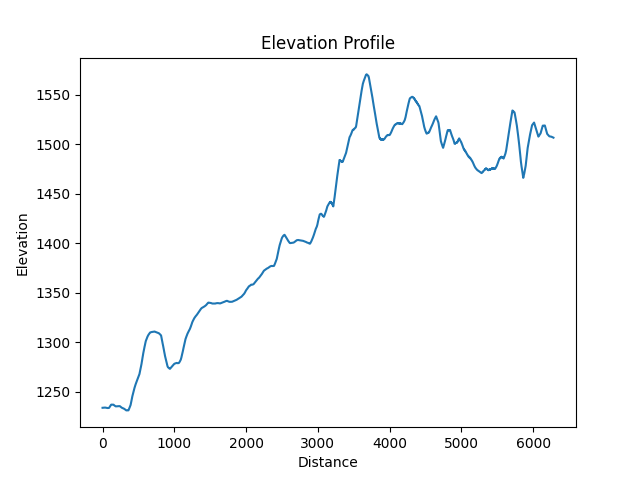
\includegraphics[width=0.3\linewidth]{elevation.png}
\caption{Plot over line \label{PlotOverCircularArcFigure}}
\end{figure}
\end{textblock*}
\end{frame}

\begin{frame}[fragile]
\begin{textblock*}{350pt}(50pt, 10pt)
\begin{block}{Extracting and Contouring}
\lstinputlisting[caption=Extracted by vector, label=WarpVectorCode, firstline=44, lastline=44]{contour.py}
\begin{figure}
\includegraphics[width=1.0\linewidth]{warped_vector.png}
\caption{Warped sphere by vector\label{WarpVectorFigure}}
\end{figure}
\end{block}
\end{textblock*}
\end{frame}
\note{
Also can have a vector filed extracted using \href{https://dev.pyvista.org/core/filters.html}{warp\_by\_vector()} method (Code List \ref{WarpVectorCode}, Figure \ref{WarpVectorFigure}).

また、 \href{https://dev.pyvista.org/core/filters.html}{warp\_by\_vector()} メソッドで抽出されたベクターファイルを持つことができます(コードリスト \ref{WarpVectorCode} 、図 \ref{WarpVectorFigure} )。

\href{https://dev.pyvista.org/plotting/plotting.html}{add\_mesh()} method can use a Matplotlib, Colorcet, cmocean, or custom colormap when plotting scalar values(Figure \ref{WarpVectorFigure}).

\href{https://dev.pyvista.org/plotting/plotting.html}{add\_mesh () }メソッドは、スカラー値をプロットするときにMatplotlib、Colorcet、cmocean、またはカスタムカラーマップを使用できます (図\ref{WarpVectorFigure}) 。

}

\begin{frame}[fragile]
\begin{textblock*}{350pt}(50pt, 10pt)
\begin{block}{Silhouette Highlight}
\lstinputlisting[caption=Silhouette Highlight, label=SilhouetteHighlight, firstline=22, lastline=28]{silhouette.py}
\begin{figure}
\includegraphics[width=1.0\linewidth]{silhouette1.png}
\caption{Silhouette Highlight\label{WarpVectorFigure}}
\end{figure}
\end{block}
\end{textblock*}
\end{frame}
\note{
We can extract a subset of the edges of a polygonal mesh to generate an outline silhouette of a mesh using add\_mesh method.
We can set it using the silhouette argument.

ポリゴンメッシュのエッジのサブセットを抽出し、add\_meshメソッドを使用してメッシュのアウトラインシルエットを生成できます。
シルエット引数で設定することができます。
}

\begin{frame}[fragile]
\begin{textblock*}{350pt}(50pt, 10pt)
\begin{block}{Back Ground Image}
\lstinputlisting[caption=Silhouette Highlight, label=SilhouetteHighlight, firstline=20, lastline=20]{background_image.py}
\begin{figure}
\includegraphics[width=1.0\linewidth]{background_image1.png}
\caption{Back Ground Image}
\end{figure}
\end{block}
\end{textblock*}
\end{frame}
\note{
We can also add background of plot using add a background image with pyvista.Plotter.add\_background\_image().
Let's Plot several earth related plots
}

\begin{frame}[fragile]
\begin{textblock*}{350pt}(50pt, 10pt)
\begin{block}{Camera class}
\begin{figure}
\includegraphics[width=0.75\linewidth]{frustum_of_camera.png}
\caption{Frustum of camera \label{CameraFrustumFigure}}
\end{figure}
\note{
\href{https://dev.pyvista.org/core/camera.html}{Camera} class is a virtual camera for 3D rendering.

\href{https://dev.pyvista.org/core/camera.html}{Camera}クラスは、3Dレンダリング用の仮想カメラです。

It provides methods to position and orient the view point and focal point.

視点や焦点の位置や方向を決めるメソッドを提供します。

Convenience methods for moving about the focal point also are provided.

また、焦点を移動するための便利なメソッドも提供されています。

More complex methods allow the manipulation of the computer graphics model including view up vector, clipping planes, and camera perspective (Figure \ref{CameraFrustumFigure}).

より複雑なメソッドでは、ビューアップベクター、クリッピングプレーン、カメラパースペクティブなど、コンピュータグラフィックスモデルを操作することができます(図 \ref{CameraFrustumFigure})。

}
\lstinputlisting[caption=Add Camera to Plotter, label=camera_view, firstline=7, lastline=13]{camera_view.py}
\end{block}
\end{textblock*}
\end{frame}

\begin{frame}[fragile]
\begin{textblock*}{350pt}(50pt, 10pt)
\begin{block}{Camera class}
\lstinputlisting[caption=Create camera frustum, label=CameraFrustumCode, firstline=8, lastline=13]{frustum_of_camera.py}
\begin{figure}
\includegraphics[width=0.75\linewidth]{camera_view.png}
\caption{Camera view}
\end{figure}
\note{
Code Listing \ref{CameraFrustumCode} create a camera and frustum.

コードリスト\ref{CameraFrustumCode}ではカメラと視錐台を作成しています。

Then create a scene of inside frustum adding \href{https://dev.pyvista.org/core/camera.html}{Camera} object to \href{https://dev.pyvista.org/plotting/plotting.html}{Plotter} object
(Code list \ref{CameraFrustumCode} ,Figure \ref{CameraFrustumFigure}).

次に、視錐台内部のシーンを作成して、\href{https://dev.pyvista.org/plotting/plotting.html}{Plotter}オブジェクトに\href{https://dev.pyvista.org/core/camera.html}{Camera}オブジェクトを追加します
(コードリスト\ref{CameraFrustumCode}、図\ref{CameraFrustumFigure})。

}
\end{block}
\end{textblock*}
\end{frame}

\begin{frame}[fragile]
\begin{textblock*}{150pt}(50pt, 10pt)
\begin{block}{Controlling Camera Rotation}
\lstinputlisting[caption=Controlling Camera Rotation, label=CameraRotationCode, firstline=29, lastline=29]{camera_view.py}
\lstinputlisting[firstline=34, lastline=34]{camera_view.py}
\lstinputlisting[firstline=39, lastline=39]{camera_view.py}
\end{block}
\end{textblock*}
\begin{textblock*}{350pt}(150pt, 50pt)
\begin{figure}
\includegraphics[width=0.5\linewidth]{camera_rotation.png}
\caption{Controlling Camera Rotation \label{CameraRotationFigure}}
\end{figure}
\note{
In addition to directly controlling the camera position by setting it via the pyvista
\href{https://dev.pyvista.org/core/camera.html}{Camera.position}
property

さらに、pyvistaの\href{https://dev.pyvista.org/core/camera.html}{Camera.position}
プロパティを使用してカメラ位置を設定することにより、カメラ位置を直接制御することもできます。

You can also directly control the
\href{https://dev.pyvista.org/core/camera.html}{pyvista.Camera.roll},
\href{https://dev.pyvista.org/core/camera.html}{pyvista.Camera.elevation}, and
\href{https://dev.pyvista.org/core/camera.html}{pyvista.Camera.azimuth}
of the camera.
(Code list \ref{CameraRotationCode} ,Figure \ref{CameraRotationFigure}).

カメラの
\href{https://dev.pyvista.org/core/camera.html}{pyvista.Camera.roll},
\href{https://dev.pyvista.org/core/camera.html}{pyvista.Camera.elevation},
および\href{https://dev.pyvista.org/core/camera.html}{pyvista.Camera.azimuth}
を直接制御することもできます。
(コードリスト\ref{CameraRotationCode}、図\ref{CameraRotationFigure})

}
\end{textblock*}
\end{frame}

\begin{frame}[fragile]
\begin{textblock*}{350pt}(50pt, 10pt)
\begin{block}{Light Types}
\lstinputlisting[caption=Headlight, label=Headlight, firstline=32, lastline=36]{light_types.py}
\begin{figure}
\includegraphics[width=1.0\linewidth]{light_types1.png}
\caption{Headlight\label{Headlight}}
\end{figure}
\end{block}
\end{textblock*}
\end{frame}
\note{
We can also set the condition of the light.
Lights come in three types:

光の状態を設定することもできます。
光源には3つのタイプがあります。

First type is headlight.
The axis of which always coincides with the view of the camera,
For headlights the position and focal\_point properties are meaningless. 
No matter where you move the camera, the light always emanates from the view point:

1つ目はヘッドライトです。
軸は常にカメラのビューと一致します。
ヘッドライトの場合、positionプロパティとfocal\_pointプロパティは意味がありません。
カメラをどこに移動しても、ライトは常に視点から放射されます。
}

\begin{frame}[fragile]
\begin{textblock*}{350pt}(50pt, 10pt)
\begin{block}{Light Types}
\lstinputlisting[caption=Cameralight, label=Cameralight, firstline=54, lastline=56]{light_types.py}
\begin{figure}
\includegraphics[width=1.0\linewidth]{light_types2.png}
\caption{Cameralight\label{Cameralight}}
\end{figure}
\end{block}
\end{textblock*}
\end{frame}
\note{
Second is camera light.
Camera lights define their position and focal\_point properties in a coordinate system that is local to the camera.
The coordinates in the scene’s coordinate system can be accessed through the world\_position and world\_focal\_point read-only properties, respectively.
For specifics of the local coordinate system used for the coordinates please see the documentation of pyvista.Light.set\_camera\_light().

2つ目はカメラライトです。カメラライトは、カメラに対してローカルな座標系で位置とfocal\_pointプロパティを定義します。
シーンの座標系の座標には、それぞれworld\_positionおよびworld\_focal\_point読み取り専用プロパティからアクセスできます。
座標に使用されるローカル座標系の詳細については、pyvistaLight.set\_camera\_light()のドキュメントを参照してください。
}

\begin{frame}[fragile]
\begin{textblock*}{350pt}(50pt, 10pt)
\begin{block}{Light Types}
\lstinputlisting[caption=Scenelight, label=Scenelight, firstline=69, lastline=71]{light_types.py}
\begin{figure}
\includegraphics[width=1.0\linewidth]{light_types3.png}
\caption{Scenelight\label{Scenelight}}
\end{figure}
\end{block}
\end{textblock*}
\end{frame}
\note{
Third is scene light.
Scene lights are attached to the scene, their position and focal point are
interpreted as global coordinates:

3つ目はシーンライトです。
シーンライトはシーンにアタッチされ、その位置と焦点はグローバル座標として解釈されます。
}

\begin{frame}[fragile]
\begin{textblock*}{350pt}(50pt, 10pt)
\begin{block}{Types of Shading}
\lstinputlisting[caption=Types of Shading, label=TypesofShading, firstline=19, lastline=23]{shading.py}
\begin{figure}
\includegraphics[width=1.0\linewidth]{shading.png}
\caption{Types of Shading\label{TypesOfShading}}
\end{figure}
\end{block}
\end{textblock*}
\end{frame}
\note{
When using lights shading is also important.
PyVista supports two types of shading, flat and smooth shading.
This is a plot with the default flat shading and smooth shading.

ライトを使用する場合は、シェーディングも重要です。
PyVistaでは、フラットシェーディングとスムーズシェーディングの2種類のシェーディングがサポートされています。
これは、既定のフラットシェーディングとスムーズシェーディングを使用したプロットです。
}

\begin{frame}[fragile]
\begin{textblock*}{350pt}(50pt, 10pt)
\begin{block}{Eye Dome Lighting}
\lstinputlisting[caption=Eye Dome Lighting, label=EyeDomeLighting, firstline=40, lastline=40]{edl.py}
\begin{figure}
\includegraphics[width=1.0\linewidth]{edl1.png}
\caption{Statue\label{Statue}}
\end{figure}
\end{block}
\end{textblock*}
\end{frame}
\note{
Eye-Dome Lighting (EDL) is a non-photorealistic, image-based shading technique designed to improve depth perception in scientific visualization images.
Eye-Dome Lighting can dramatically improve depth perception when plotting incredibly sophisticated meshes like the creative commons Queen Nefertiti statue:
Here we will compare a EDL shading side by side with normal shading

アイドームライティング (EDL) は、科学的可視化イメージの奥行き知覚を改善するために設計された、非フォトリアリスティックなイメージベースのシェーディングテクニックです。
アイドームライティングは、クリエイティブ・コモンズのネフェルティティ女王の像のような非常に洗練されたメッシュを描画するときに、奥行きの知覚を劇的に改善します。
ここでは、EDLシェーディングと通常のシェーディングを並べて比較します。
}

\begin{frame}[fragile]
\begin{textblock*}{350pt}(50pt, 10pt)
\begin{block}{Eye Dome Lighting}
\lstinputlisting[caption=Eye Dome Lighting, label=EyeDomeLighting, firstline=40, lastline=40]{edl.py}
\begin{figure}
\includegraphics[width=1.0\linewidth]{edl2.png}
\caption{Point Cloud\label{PointCloud}}
\end{figure}
\end{block}
\end{textblock*}
\end{frame}
\note{
When plotting a simple point cloud, it can be difficult to perceive depth.
Take this Lidar point cloud for example.
And now plot this point cloud as-is.

単純な点群を印刷する場合、奥行きを認識するのが難しいことがあります
たとえば、このライダー点群を考えてみましょう。
次に、この点群をそのまま描画します。
}

\begin{frame}[fragile]
\begin{textblock*}{350pt}(50pt, 10pt)
\begin{block}{Applying Textures}
\lstinputlisting[caption=Applying Textures, label=EyeDomeLighting, firstline=27, lastline=29]{texture.py}
\begin{figure}
\includegraphics[width=1.0\linewidth]{texture1.png}
\caption{Applying Textures\label{ApplyingTextures}}
\end{figure}
\end{block}
\end{textblock*}
\end{frame}
\note{
We can also plot a mesh with an image projected onto it as a texture.
Texture mapping is easily implemented using PyVista.
Many of the geometric objects come preloaded with texture coordinates, so quickly creating a surface and displaying an image is simple.

また、イメージをテクスチャとして投影したメッシュをプロットすることもできます。
テクスチャマッピングは、PyVistaを使用して簡単に実装できます。
ジオメトリックオブジェクトの多くにはテクスチャ座標があらかじめロードされているため、サーフェスをすばやく作成してイメージを表示するには、次の操作を実行します。
}

\begin{frame}[fragile]
\begin{textblock*}{350pt}(50pt, 10pt)
\begin{block}{Physically Based Rendering (PBR)}
\lstinputlisting[caption=Physically Based Rendering (PBR), label=PBR, firstline=35, lastline=37]{pbr.py}
\begin{figure}
\includegraphics[width=1.0\linewidth]{pbr1.png}
\caption{Physically Based Rendering (PBR) Textures\label{PBRFigure}}
\end{figure}
\end{block}
\end{textblock*}
\end{frame}
\note{

VTK 9 introduced Physically Based Rendering (PBR) and we have exposed that functionality in PyVista.
PBR is only supported for pyvista.PolyData and can be triggered via the pbr keyword argument of add\_mesh.
Also use the metallic and roughness arguments for further control.
Let’s show off this functionality by rendering a high quality mesh of a statue as though it were metallic.
Let’s render the mesh with a base color of “linen” to give it a metal looking finish.

VTK 9はPhysically Based Rendering (PBR) を導入し、その機能をPyVistaで公開しました。
PBRは、pyvistaでのみサポートされています。PolyDataであり、add\_meshのpbrキーワード引数を介してトリガできます。
さらにコントロールするには、metallic引数とroughness引数も使用します。
ここでは、彫像の高品質のメッシュをメタリックであるかのようにレンダリングして、この機能を紹介します。
メッシュを 「リネン」 のベースカラーでレンダリングして、金属のような仕上げにします。
}

\begin{frame}[fragile]
\begin{textblock*}{350pt}(50pt, 10pt)
\begin{block}{Physically Based Rendering (PBR)}
\lstinputlisting[caption=Physically Based Rendering (PBR), label=PBR, firstline=35, lastline=37]{pbr.py}
\begin{figure}
\includegraphics[width=1.0\linewidth]{pbr2.png}
\caption{Physically Based Rendering (PBR) Textures\label{PBRFigure}}
\end{figure}
\end{block}
\end{textblock*}
\end{frame}
\note{

This figure show the variation of the metallic and roughness parameters.
Plot with metallic increasing from left to right and roughness increasing from bottom to top.

この図は金属と粗さのパラメータの変化を示しています。
左から右に向かって金属の属性が増加し、下から上に向かって粗さが増加するようにプロットしています。

}

\begin{frame}[fragile]
\begin{textblock*}{350pt}(50pt, 10pt)
\begin{block}{Box Widget}
\lstinputlisting[caption=Box Widget, label=BoxWidgetList, firstline=30, lastline=32]{box-widget.py}
\end{block}
\begin{figure}
\movie[width=5cm,height=5cm]{}{box-clip.gif}
\end{figure}
\end{textblock*}
\end{frame}
\note{
PyVista has several widgets that can be added to the rendering scene to control filters like clipping, slicing, and thresholding.
The box widget can be enabled and disabled by the pyvista.WidgetHelper.add\_box\_widget() and pyvista.WidgetHelper.clear\_box\_widgets() methods respectively.
When enabling the box widget, you must provide a custom callback function otherwise the box would appear and do nothing - the callback functions are what allow us to leverage the widget to perform a task like clipping/cropping.
Considering that using a box to clip/crop a mesh is one of the most common use cases, we have included a helper method that will allow you to add a mesh to a scene with a box widget that controls its extent, the pyvista.WidgetHelper.add\_mesh\_clip\_box() method.

PyVistaには、クリッピング、スライス、しきい値などのフィルタを制御するためにレンダリングシーンに追加できるウィジェットがいくつかあります。
ボックスウィジェットは、ピビスタで有効または無効にできます。WidgetHelper.add\_box\_widget () およびpyvista。それぞれWidgetHelper.clear\_box\_widgets () メソッド。
ボックスウィジェットを有効にするときは、カスタムコールバック関数を提供する必要があります。
そうしないと、ボックスが表示されて何も実行されません。
コールバック関数を使用すると、ウィジェットを利用してクリッピングやクロップなどのタスクを実行できます。

}

\begin{frame}[fragile]
\begin{textblock*}{350pt}(50pt, 10pt)
\begin{block}{Plane Widget}
\lstinputlisting[caption=Plane Widget, label=PlaneWidgetList, firstline=23, lastline=25]{plane-widget.py}
\end{block}
\begin{figure}
\movie[width=5cm,height=5cm]{}{plane-clip.gif}
\end{figure}
\end{textblock*}
\end{frame}
\note{
The plane widget can be enabled and disabled by the pyvista.WidgetHelper.add\_plane\_widget() and pyvista.WidgetHelper.clear\_plane\_widgets() methods respectively.
As with all widgets, you must provide a custom callback method to utilize that plane.
Considering that planes are most commonly used for clipping and slicing meshes, we have included two helper methods for doing those tasks!

プレーンウィジェットは、pyvista.WidgetHelper.add\_plane\_widget()とpyvista.WidgetHelper.clear\_plane\_widgets()で有効または無効にできます。
すべてのウィジェットと同様に、そのプレーンを利用するカスタムコールバックメソッドを提供する必要があります。
平面はメッシュのクリッピングとスライスに最も一般的に使用されることを考慮して、これらのタスクを実行する2つのヘルパーメソッドを用意しました。
}

\begin{frame}[fragile]
\begin{textblock*}{350pt}(50pt, 10pt)
\begin{block}{Slider Widget}
\lstinputlisting[caption=Slider Widget, label=SliderWidgetList, firstline=26, lastline=28]{slider-bar-widget.py}
\end{block}
\begin{figure}
\movie[width=5cm,height=5cm]{}{plane-clip.gif}
\end{figure}
\end{textblock*}
\end{frame}
\note{
The slider widget can be enabled and disabled by the pyvista.WidgetHelper.add\_slider\_widget() and pyvista.WidgetHelper.clear\_slider\_widgets() methods respectively.
This is one of the most versatile widgets as it can control a value that can be used for just about anything.

スライダウィジェットは、pyvistaでWidgetHelper.add\_slider\_widget ()および有効または無効にできます。
これは、ほぼすべての目的に使用できる値を制御できるため、最も用途の広いウィジェットの1つです。
}

\begin{frame}[fragile]
\begin{textblock*}{350pt}(50pt, 10pt)
\begin{block}{Sphere Widget}
\lstinputlisting[caption=Single Sphere Widget, label=SphereWidgetList, firstline=37, lastline=39]{sphere-widget.py}
\end{block}
\begin{figure}
\movie[width=5cm,height=5cm]{}{sphere-widget-a.gif}
\end{figure}
\end{textblock*}
\end{frame}
\note{
The sphere widget can be enabled and disabled by the pyvista.WidgetHelper.add\_sphere\_widget() and pyvista.WidgetHelper.clear\_sphere\_widgets() methods respectively.
This is a very versatile widget as it can control vertex location that can be used to control or update the location of just about anything.
We don’t have any convenient helper methods that utilize this widget out of the box, but we have added a lot of ways to use this widget so that you can easily add several widgets to a scene.
Let’s look at a few use cases that all update a surface mesh.
This example Use a single sphere widget

球ウィジェットは、 pyvista.WidgetHelper.add\_sphere\_widget() と  pyvista.WidgetHelper.clear\_sphere\_widgets() で有効または無効にできます。
これは頂点の位置を制御できるため、非常に用途の広いウィジェットで、ほぼすべての位置の制御や更新に使用できます。
このウィジェットをそのまま使用する便利なヘルパーメソッドはありませんが、シーンに複数のウィジェットを簡単に追加できるように、このウィジェットを使用する方法が多数追加されています。
サーフェスメッシュを更新するいくつかの使用例を見てみましょう。
これは単体の球ウィジェットの例です。
}

\begin{frame}[fragile]
\begin{textblock*}{350pt}(50pt, 10pt)
\begin{block}{Sphere Widget}
\lstinputlisting[caption=Several Sphere Widget, label=SeveralSphereWidgetList, firstline=69, lastline=71]{sphere-widget.py}
\end{block}
\begin{figure}
\movie[width=5cm,height=5cm]{}{sphere-widget-b.gif}
\end{figure}
\end{textblock*}
\end{frame}
\note{
Use several sphere widgets at once.
Check that callback function is different.

1度に複数の球ウィジェットを使用します。
コールバック関数が異なることに注意してください。
}

\begin{frame}[fragile]
\begin{textblock*}{350pt}(50pt, 10pt)
\begin{block}{Acknowlegment}
I would like to thank \href{https://github.com/orgs/pyvista/teams/developers}{PyVista developer team} for developing useful library.
\end{block}
\begin{block}{References}
C. Bane Sullivan and Alexander Kaszynski, (2019). PyVista: 3D plotting and mesh analysis through a streamlined interface for the Visualization Toolkit (VTK). Journal of Open Source Software, 4(37), 1450, \url{https://doi.org/10.21105/joss.01450}
\end{block}
\begin{block}{Contact Information}
If you want to know and discuss pyvista more, join \href{http://github.com/pyvista/pyvista/discussions}{GitHub Discussion}.
\end{block}
\doclicenseThis
\end{textblock*}
\end{frame}
\note{
I would like to thank PyVista developer team for developing useful library.

役に立つライブラリを開発してくれたPyVista開発チームに感謝します。

If you want to know and discuss pyvista more, join \href{http://github.com/pyvista/pyvista/discussions}{GitHub Discussion}.

pyvistaについてもっと知りたいなら、\href{http://github.com/pyvista/pyvista/discussions}{GitHub Discussion}に参加してください。

}

\end{document}

